\documentclass{beamer-control}
\usepackage{beamer-control-singlefile}
\INCLUDEONLY{Welcome}
\begin{document}

\lecture{Welcome}{Welcome}

\begin{frame}[plain]
\def\currCONCEPT{Welcome to the course}
\def\insertsubsectionnumber{0}
\usebeamertemplate{subsection page}
\end{frame}

\begin{frame}
\frametitle{Welcome to Applied Control Systems}
\framesubtitle{An applied but rigorous introduction to control systems for mechanical engineers}

\emph{We hope the course will open your mind and teach practical skills!}
\bigskip

\begin{itemize}
\item What are the learning activities?
\item What is the assessment?
\item What are the requirements?
\end{itemize}
\end{frame}

\begin{frame}
\frametitle{What are the learning activities?}
\begin{itemize}
\item Read the textbook (!)
\item Watch the recorded videos
\item Attend the workshop (computer session---theory)
\item Attend the practical (laboratory---practice)
\end{itemize}
\end{frame}


\begin{frame}
\frametitle{What is the assessment?}
\begin{itemize}
\item Formative quizzes
\item Assignments $\times$3 (15\%)
\item Practical workbooks $\times3$ (non-graded pass)
\item Practical project report (25\%)
\item Exam (60\%)
\end{itemize}
\end{frame}

\begin{frame}
\frametitle{What are the requirements?}
\begin{itemize}
\item Matlab
\item Simulink
\item Mobius for assignments, exam
\item Practical attendance, exam attendance
\end{itemize}
\end{frame}

\begin{frame}
\centering
\Large \alert{Introduction to the textbook}
\end{frame}

\begin{frame}
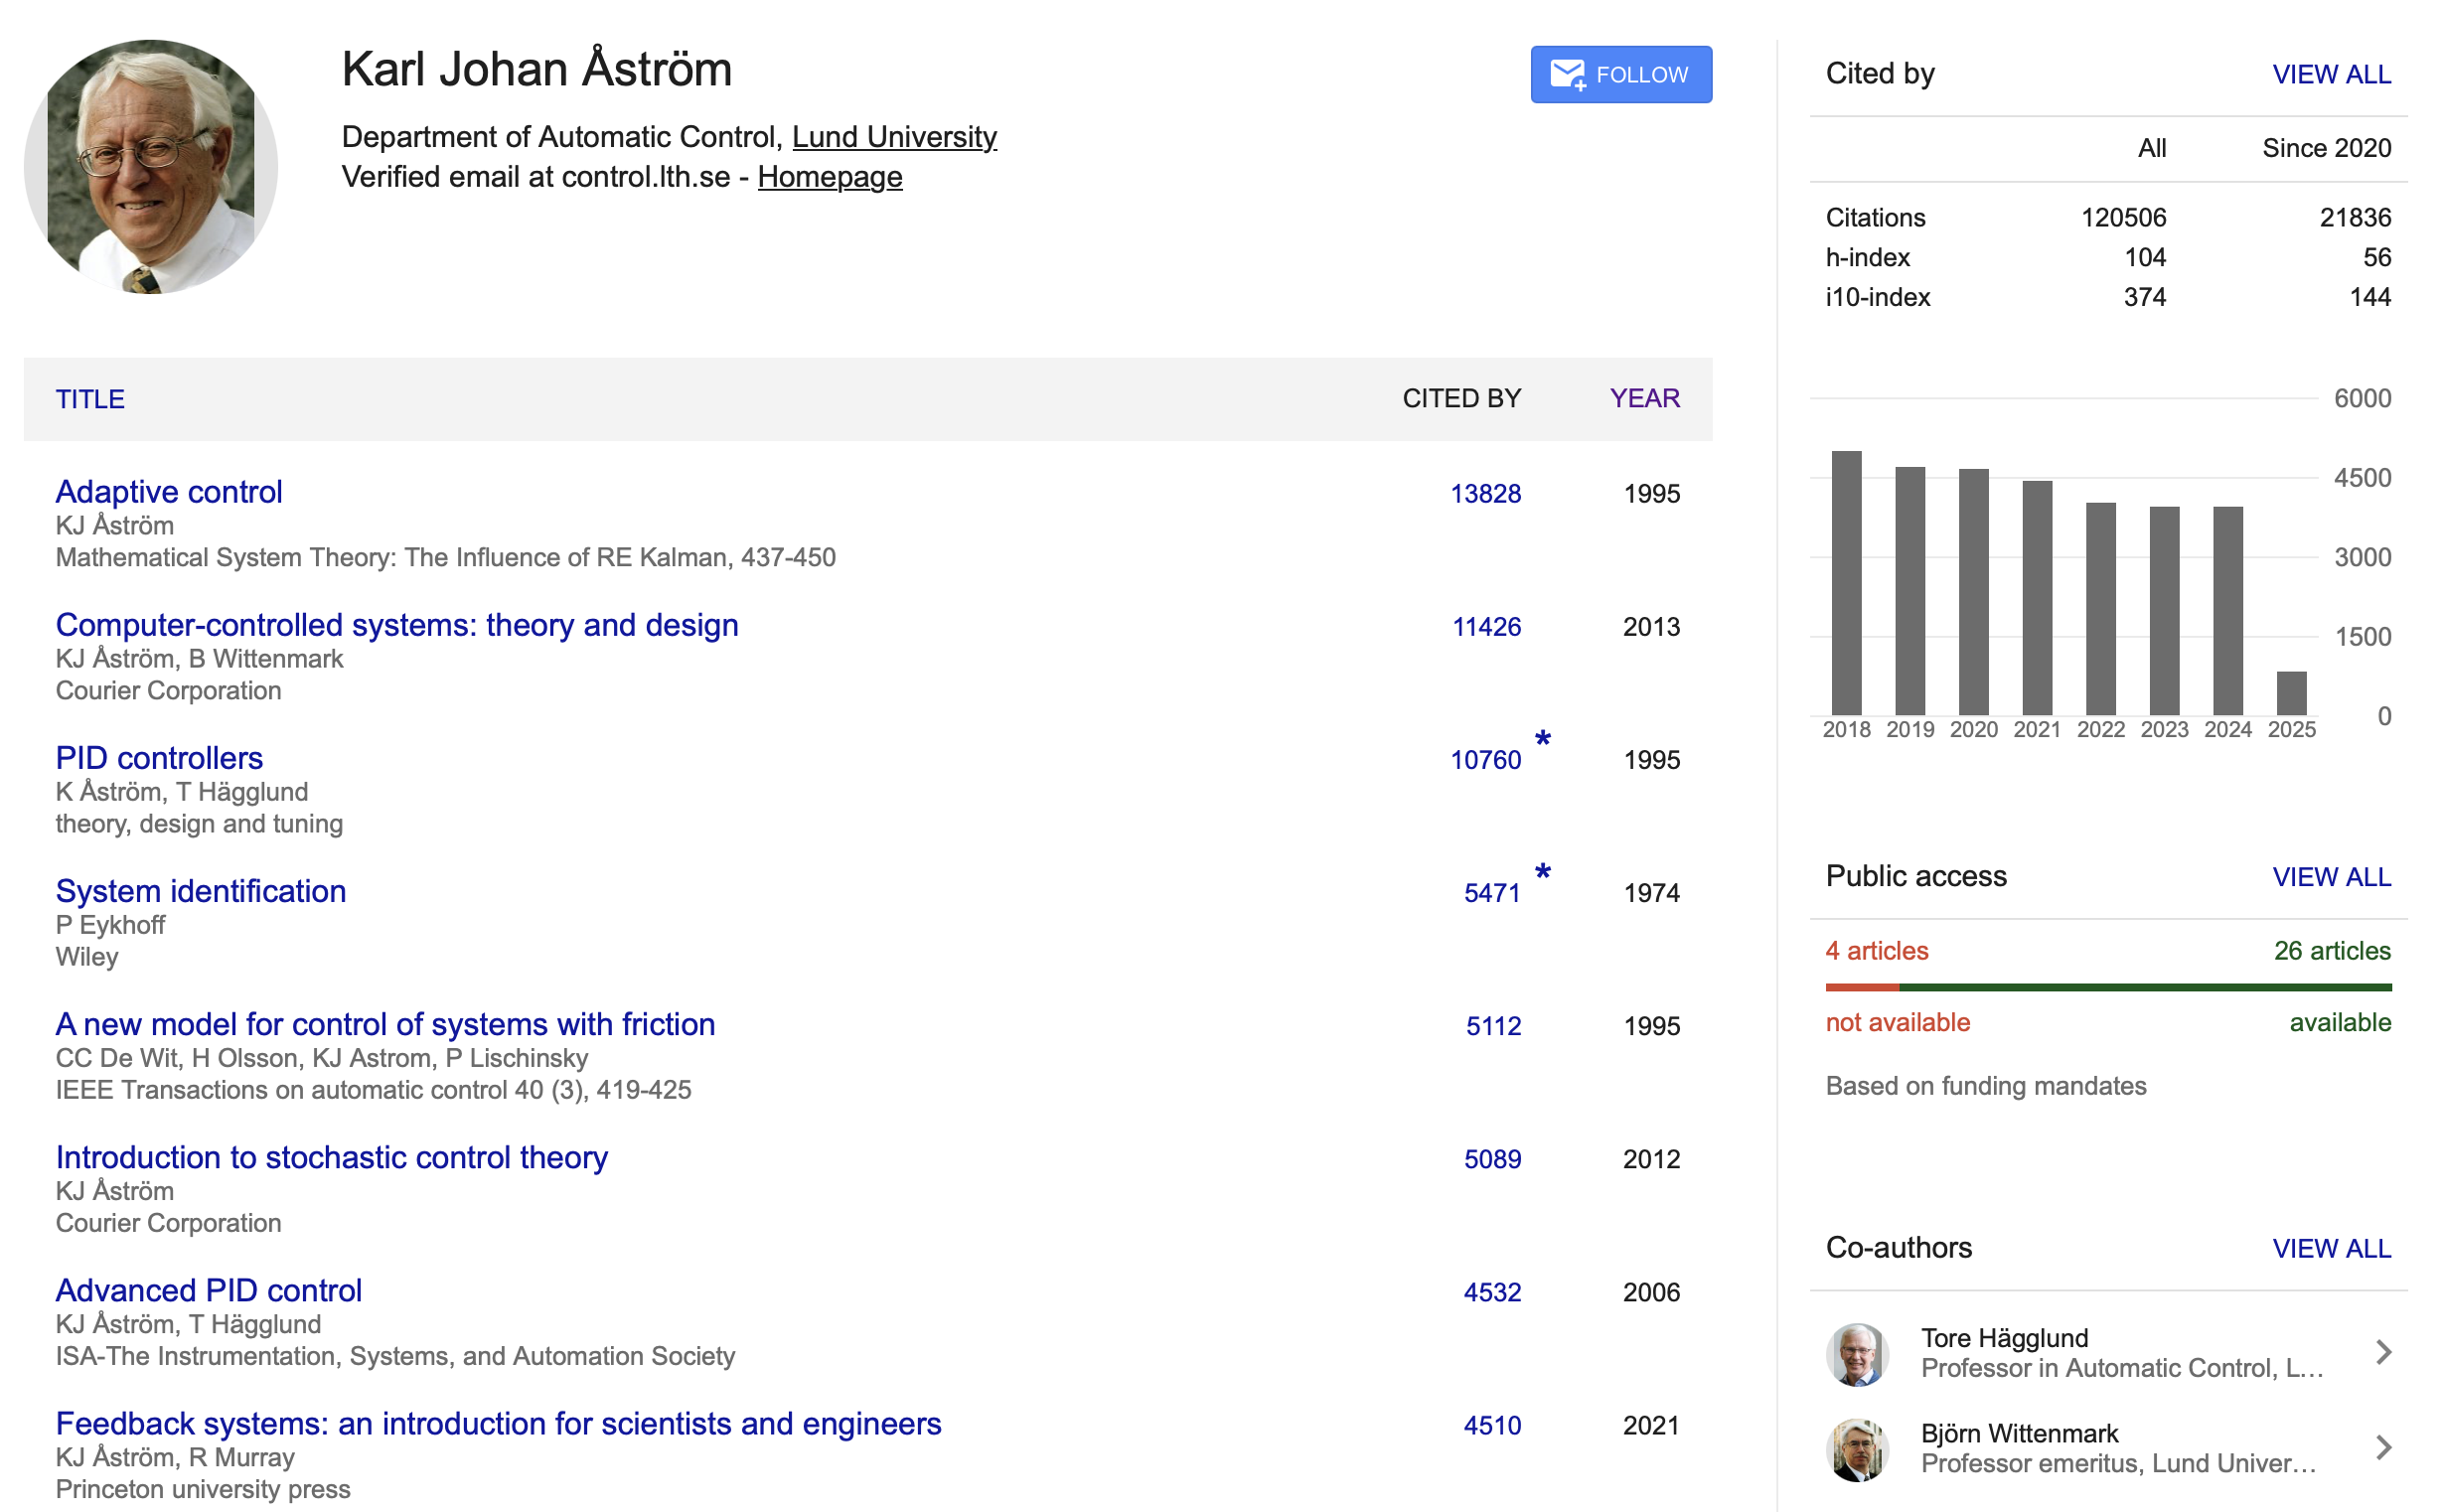
\includegraphics[width=\linewidth]{astrom}
\end{frame}

\begin{frame}
\frametitle{The course material}
\begin{itemize}[<uncover@+->]
\item Textbook: `\emph{Feedback Systems: An Introduction for Scientists and Engineers}' by Åström \& Murray, 2nd edition.
\item The textbook is perfect for our curriculum:
\begin{itemize}
\item 10 week course, omitting some technical sections
\item No assumption of a `signals and systems' background (Laplace Transforms)
\item Rigorous yet practical with many cross-disciplinary examples
\end{itemize}
\end{itemize}
\end{frame}

\begin{frame}
\frametitle{Course modules and topics}
\small

\centerline{%
\begin{tabular}{>{\hangindent=1em\raggedright\arraybackslash}l>{\hangindent=1em\raggedright\arraybackslash}p{5cm}l}
\toprule
Module & Topic & \S \\
\midrule
Dynamical Systems & Introduction and System Modelling & Ch.1,3 \\ 
& Dynamic Behaviour & Ch.4,5 \\ 
& Linear Systems & Ch.6 \\\midrule
Control System Concepts & State Feedback & Ch.7 \\ 
& Transfer Functions& Ch.9 \\ 
& Frequency Domain Analysis& Ch.10 \\\midrule
Control System Design & PID Control& Ch.11 \\ 
& Frequency Domain Design& Ch.12 \\ 
& Robust Performance \& Fundamental Limits& Ch.13,14  \\
\bottomrule
\end{tabular}}
\end{frame}

\FINALE

\end{document}
